Betrachten Sie folgendes Petrinetz:



\begin{centering}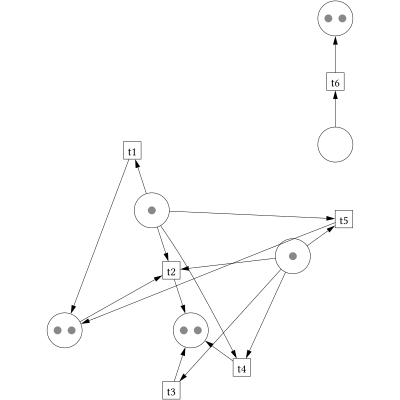
\includegraphics[min width=0.4\textwidth=0.6\textwidth,min height=0.4\textwidth=0.6\textwidth,keepaspectratio,max width=0.9\textwidth,max height=0.9\textwidth]{63/concurrentpetri7d70a8768ee1cdf2002c8d703dde2d744fda5473affcaeb8018a96c73a31bf8d01012.pdf}\end{centering}

Welches Paar von Transitionen ist unter der Startmarkierung nebenläufig aktiviert?

Geben Sie Ihre Antwort durch Angabe eines Paars von nebenläufig aktivierten Transitionen an.  Die Angabe von \begin{verbatim}(t0,t1)\end{verbatim} als Antwort würde bedeuten, dass Transitionen t0 und t1 unter der Startmarkierung nebenläufig aktiviert sind.  Die Reihenfolge der Transitionen innerhalb des Paars spielt hierbei keine Rolle.

Bitte beachten Sie: Beim Bewegen über oder Klicken auf Kanten / Knoten bzw. ihre Beschriftungen werden die jeweils zusammengehörenden Komponenten hervorgehoben.

